%!TEX root = ../maturaarbeit.tex


\section{Aufbau von Galaxien}
Es gibt verschiedene Arten von Galaxien, wie zum Beispiel die elliptische-, spiral-, balken-,\\ linsenförmige-, und die irreguläre Galaxien. Sie unterscheiden sich in Struktur und Form. 
Grundsätzlich haben alle Galaxien ein Gravitationszentrum, um das sich die gesammte Galaxie dreht. Im Zentrum der Galaxie befindet sich ein schwarzes Loch, welches von einem sogenannten Bulge umgeben ist. 
Dieser Bulge ist eine riesige Sternenansammlung auf relativ engem Raum. Um das Zentrum herum erstreckt sich eine galaktische Scheibe, in der sich die meisten Sterne, interstellares Gas und Staub befinden.
Je nach Art der Galaxie sind die Arme der Galaxie anders angeordnet, zum Beispiel sind diese spiralförmig in der Spiralgalaxie.\\ Um die Scheibe herum befindet sich ein sphärischer Halo, in dem sich Sterne und Kugelsternhaufen befinden \cite{Ribas2020}.  
Im Bild unten ist der Seitenriss vom Aufbau der Milchstrasse zu erkennen. Im Zentrum befindet sich das schwarze Loch, umgeben vom Bulge, welches sich inmitten der Galaxiescheibe befindet. Auf dem Bild ist zusätzlich unsere Sonne markiert.

\begin{figure}[H]
	\centering
	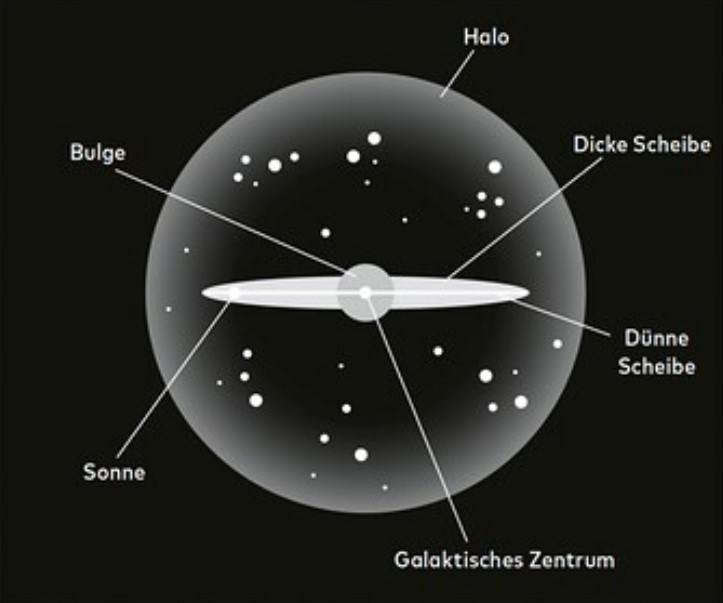
\includegraphics[width=0.4\textwidth]{figures/aufbau_galaxie.jpg}
	\caption[Abbildung 1: Aufbau Milchstrasse]{Aufbau der Milchstrasse \cite{Anderl2023}}
	\label{fig Aufbau Galaxie}
\end{figure}


\subsection{Die Rotationskurve}

Rotationskurven geben an, wie sich die Geschwindigkeit von Objekten innerhalb einer Galaxie im Vergleich zum Abstand vom Zentrum verändern. 
Damit die Rotationskurve und die Massenverteilung von Galaxien berechnet werden können, müssen ihre Strukturen sowie ihre Zusammensetzungen aus Sternen, Staub, stellarem Gas und Dunkler Materie bekannt sein \cite{Moeller2010}. 

Die universale Rotationskurve ist eine mathematische Formel, die die Rotationskurven von Galaxien anhand ihrer Gesamthelligkeit und ihres Radius charakterisiert.
Dadurch kann darauf geschlossen werden, dass die hellsten Galaxien eine leicht abfallende Rotationskurve haben, mittlere Galaxien eine konstant flache und dunklere Galaxien eine monoton ansteigende Rotationskurve \cite{SofueVera2000}. 
Auf dem Bild ist die Art der Rotationskurve, die man bei Spiralgalaxien erwarten würde, zu sehen aufgrund der Verteilung der Sterne, dargestellt durch die gestrichelete Linie. Sie steht im Vergleich zu den gemessenen Geschwindigkeiten.
\begin{figure}[H]
	\centering
	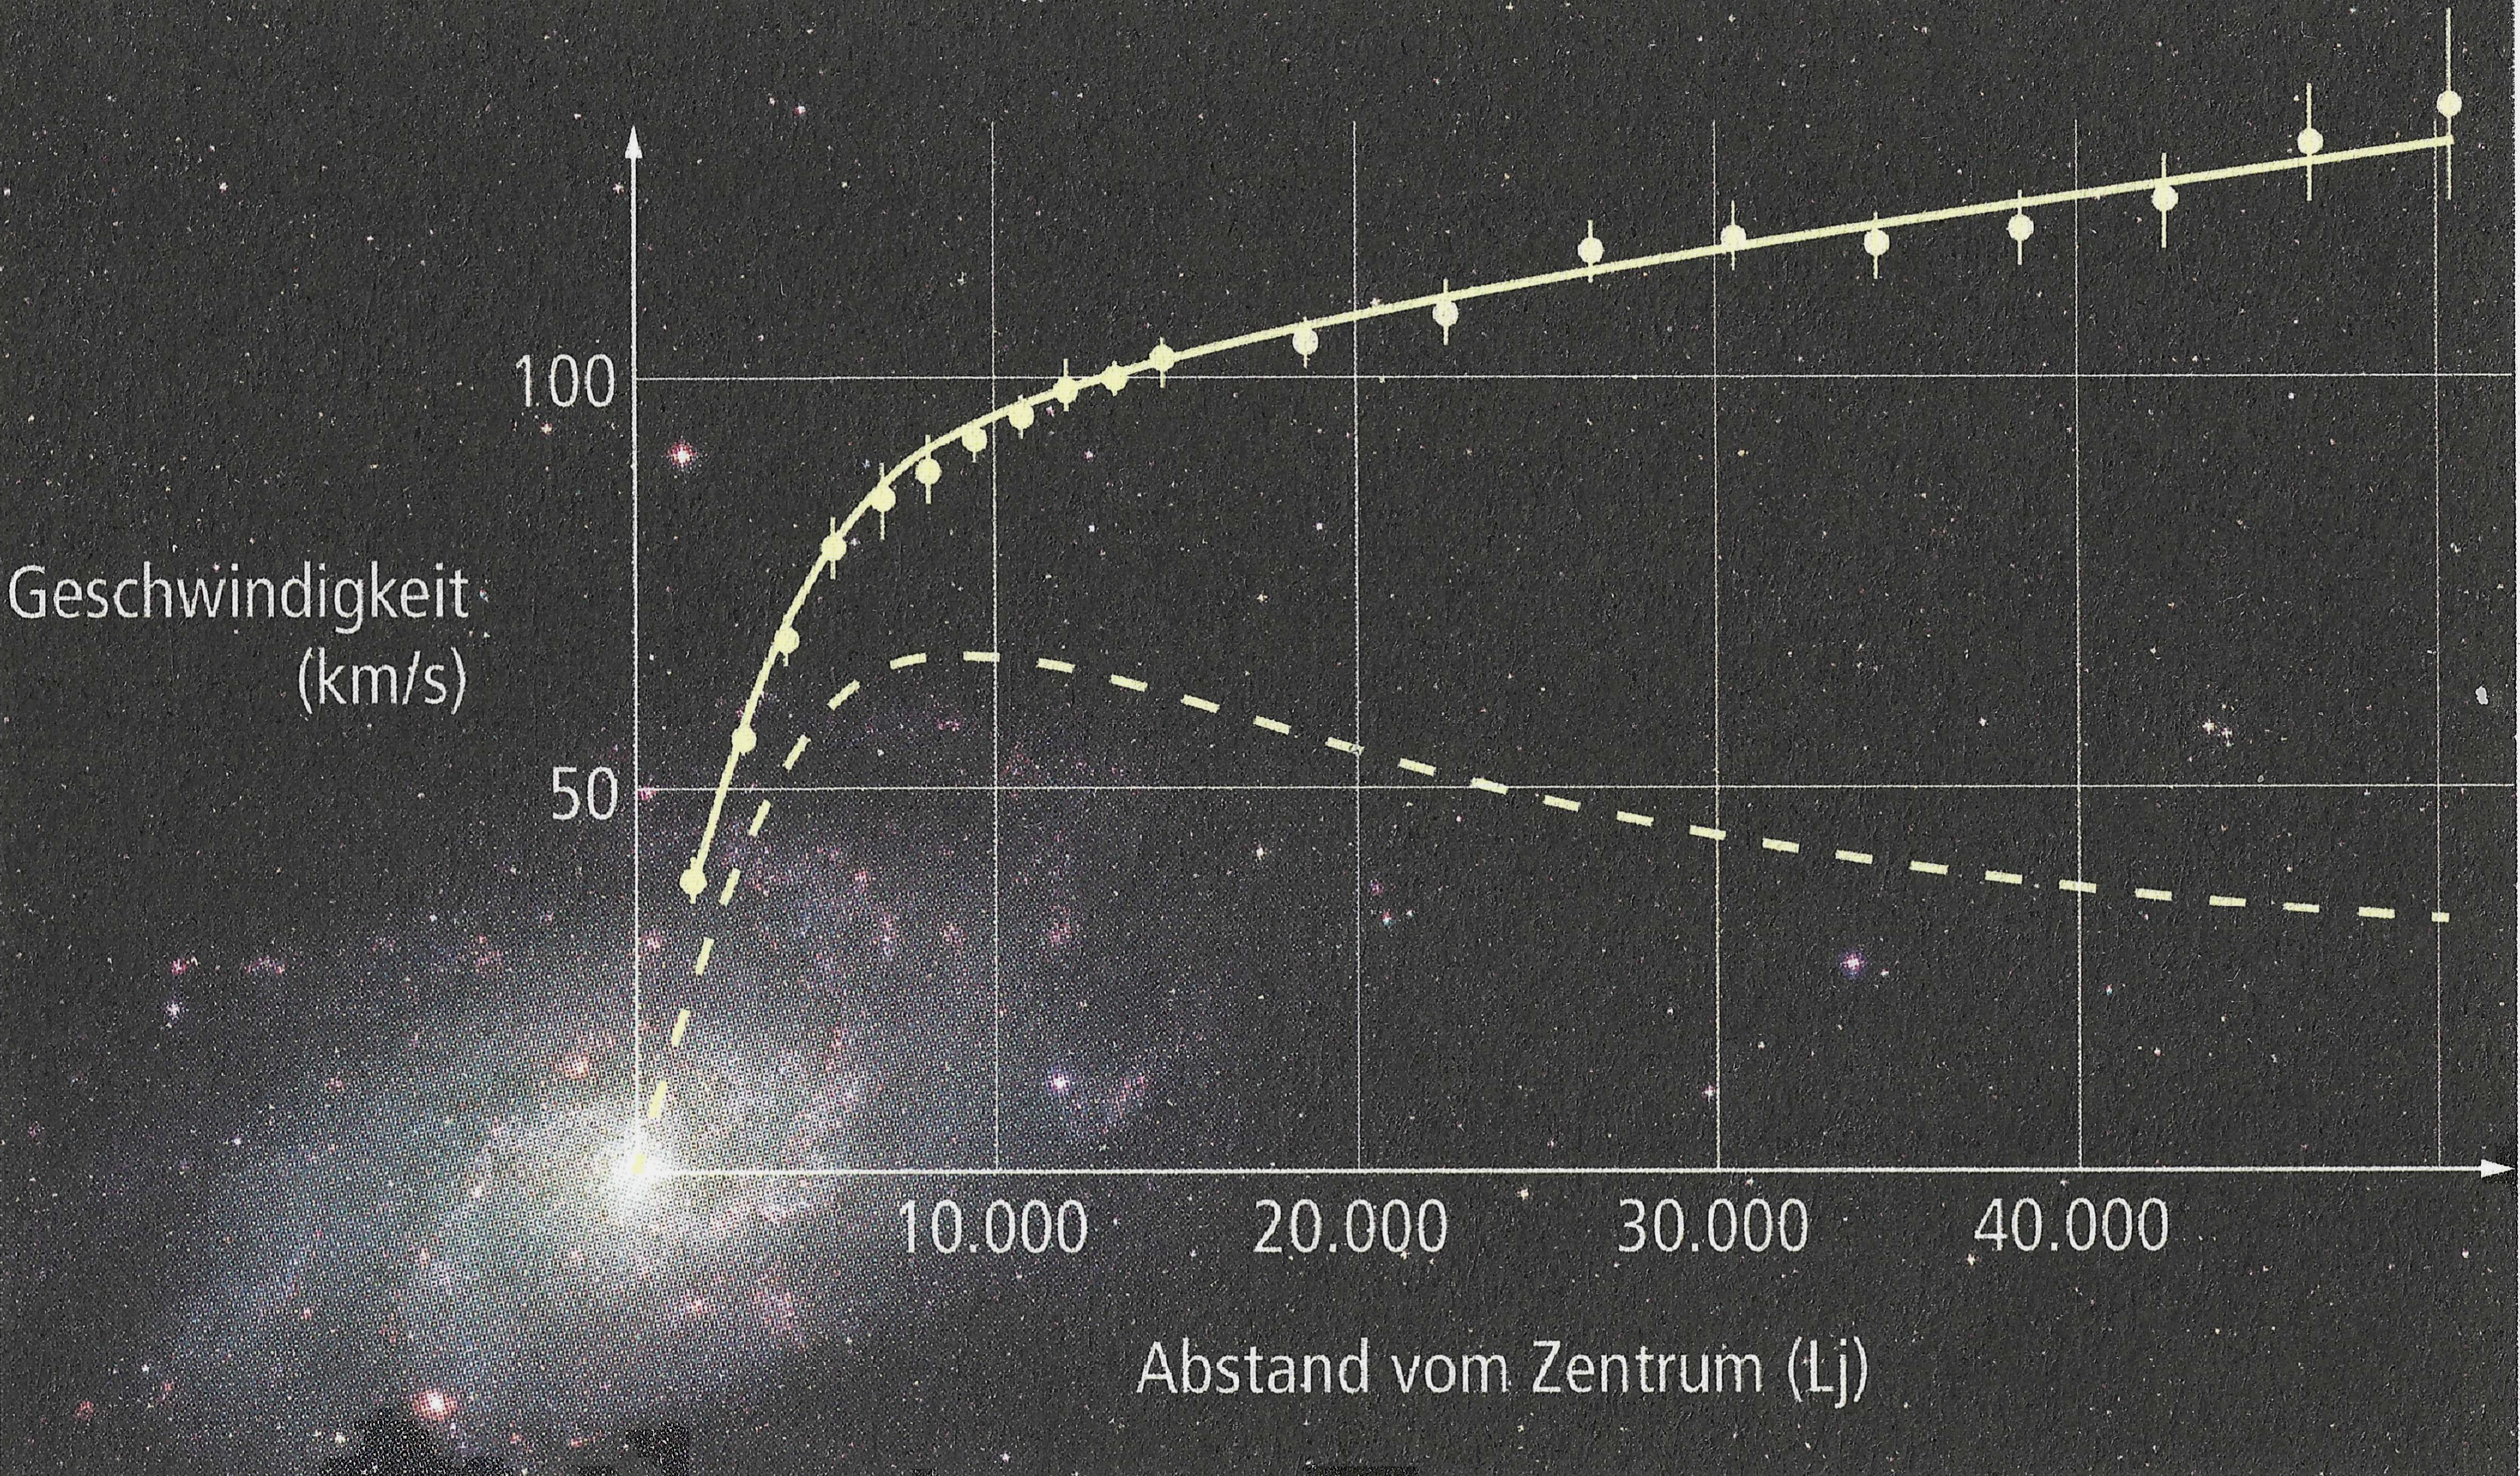
\includegraphics[width=0.6\textwidth]{figures/right_curve.jpg}
	\caption[Abbildung 2: Berechnete und beobachtete Rotationskurve ]{Berechnete und gemessene Rotationskurve der Galaxie Messier 33 \cite{Bührke2022}}
	\label{fig Rotationskurve.}
\end{figure}

\subsection{Galaxien drehen zu schnell}
(ganzes Kapitel nach \cite{Bührke2022})\\
Die Formel zu Berechnung von der Orbitalgeschwindigkeit lautet:
\begin{align*}    
    v = \sqrt[2]{\frac{G \cdot M}{r}}
\end{align*}
G ist die Gravitationskonstante, M die Masse des Zentralobjektes und r die Distanz zwischen den Objekten. Bei M muss beachtet werden, dass die gesamte Masse innerhalb der jeweiligen Planetenbahn zählt. 
Von dieser Formel kann darauf geschlossen werden, dass sich das Objekt langsamer bewegt, je weiter weg es sich vom Zentrum befindet. Das trifft auch bei den Planeten in unserem Sonnensystem zu, da durch r dividiert wird.
Dieses Gesetz kann auf alle Systeme, wo ein Körper einen Zentralbereich umkreist, angewendet werden. \\Ähnlich ist es bei Galaxien. Im Zentrum der Galaxie befindet sich nicht eine einzige dominierende Masse, sondern der sogenannte Bulge. 
Dort befinden sich so viele Sterne, dass sie nicht mehr einzeln zu erkennen sind.\\ Mit der Spektroskopie, einer Technik bei der Licht in die verschiedenen Wellenlängen oder Frequenzen aufgeteilt wird, der fernen Sternsysteme können Aufschlüsse über die Bewegungen und Masse der Sterne gezogen werden.
Jedoch erweist sich die Aufnahme von Spektren als Herausforderung, vor allem die Bestimmung der Geschwindigkeit von Objekten in den lichtschwachen Aussenbereichen der Scheibe. Vergleicht man die hellen Zentralgebiete mit den äusseren Gebieten, sind dort nicht mehr viele Sterne zu erwarten. 
Daraus lässt sich der Schluss ziehen, dass die Geschwindigkeit mit zunehmendem Abstand vom Zentrum abnehmen muss, ähnlich wie im Sonnensystem.\\
Jedoch beobachtete Horace Babcock im Jahr 1939, der mit einem neuen Spektrografen die Rotationskurve der Andromeda-Galaxie mass, etwas Überaschendes. Anstelle einer abfallenden Rotationskurve blieb sie bis in die Aussenbereiche konstant, sie schien sogar eher zuzunehmen.

Wenn die Geschwindigkeit der Körper mit wachsendem Abstand vom Zentrum nicht abnimmt, sondern konstant bleibt, muss sich innerhalb der Umlaufbahn unsichtbare Materie befinden, welche eine erhebliche Schwerkraft ausübt. Vereinfacht ausgedrückt: Galaxien haben zu wenig Masse, als dass sie sich so schnell drehen könnten.
Für ein besseres Verständnis kann man sich ein Kettenkarussell vorstellen, dessen Sessel sich so schnell drehen, dass die Ketten reissen. Jedoch halten die Spiralgalaxien aus unerklärlichen Gründen zusammen.\\
Der Astronom Jan Hendrik Oort stiess im selben Jahr auf das gleiche Problem, als er Daten von der Galaxie NGC 3115 auswertete. Diese Galaxie zählt zu den linsenförmigen, mit einem zentralen Bulge und einer ausgeprägten Scheibe ohne Spiralarme.
Oort kam wie Babcock, der in der Andromeda Galaxie zu hohe Geschwindigkeiten der Objekte weit vom Zentrum entfernt mass, auf dasselbe Ergebnis. Die Umlaufgeschwindigkeiten der Sterne nehmen mit wachsendem Abstand vom Zentrum nicht ab. 
Oort kam zum Schluss, dass die Massenverteilung fast keine Beziehung zu der des Lichts habe. Er vermutete, dass es sehr lichtschwache und damit nicht mehr erkennbare Zwergsterne geben müsse, welche eine Erklärung für die fehlende Masse wäre.\\
Vera Rubin, eine der ersten Frauen, die sich in dieser zu der Zeit männerdominierten Forschungsrichtung durchsetzte, beobachtete die Geschwindigkeit von etwa 1000 Sternen in der Milchstrasse und kam 1965 zu demselben Schluss: Die Rotationskurve ist flach und nimmt nicht ab, wie es erwartet worden wäre.\\
Obwohl viele Wissenschaftler/innen zu demselben Schluss kamen, nämlich einer zu schnellen Rotationskurve von Galaxien, zweifelten viele an diesen Ergebnissen. Erst 1971, als die Messgeräte besser wurden und dadurch auch die Messdaten genauer, wurden Lösungen für dieses Problem gesucht. 
Eine erste Vermutung war eine grosse Menge an Zwergsternen in den äusseren Bereichen der Galaxien, diese wären somit nicht mehr erkennbar. Jedoch ergab sich dadurch die Frage, warum sich ausschliesslich nur Zwergsterne in den Aussenbereichen befinden und keine helleren Sterne, welche erkennbar sein müssten.\\
1970 stiess Frank Hohl auf ein weiters Problem mit den zu hohen Drehgeschwindigkeiten von Galaxien. Er simulierte die Sternensysteme einer Spiralgalaxie mit theoretischen Masseteilchen, unter Einfluss der Gravitation. 
Nach wenigen Umdrehungen wurde die Galaxiescheibe instabil, die Sterne brachen aus ihren Kreisbahnen und die Spiralgalaxie verformte sich in eine balkenartige Struktur. Jedoch kann von der Häufigkeit von Spiralgalaxien im Universum darauf geschlossen werden, dass dies nicht zutrifft, Spiralgalaxien behalten ihre Form.\\
Auf eine mögliche Lösung für die Instabilität und die fehlende Materie von Galaxien kamen 1972 James Peebles, Jeremiah Ostriker und Jaan Einasto; Galaxien mussten von einer riesigen Wolke aus unsichtbarer Dunkler Materie umgeben sein, einem sogenannten Halo oder einer Korona aus Dunkler Materie. Dieser Halo müsste zweieinhalbmal mehr Materie enthalten als die Galaxie selbst.\\  
Es gibt auch Wissenschaftler/innen und Wissenschaftler, die an der Existenz Dunkler Materie zweifeln. Sie sehen nicht den Fehler in den zu schnellen Rotationskurven, sondern in den newtonschen Gravitationsgesetzen, die verwendet werden, um die Rotationskurven zu berechnen. Mordehai Milgrom entwickelte deshalb eine alternative Gravitationstheorie, die \glqq MOND\grqq{} (\glqq MOdified Newtonian Dynamics\grqq{}) genannt wird, was für \glqq Modifizierte Newtonsche Dynamik\grqq{} steht.
Diese modifizierte Theorie kann zwar das Phänomen der zu schnellen Rotationskurven ohne die Existenz von Dunkler Materie erklären, weist jedoch auch viele Probleme auf. Zum Beispiel lässt sich mit dieser Theorie die Entstehung der Galaxien aus dem Urgas nicht erklären.\\
Seit dem Einsatz des Weltraumteleskops Gaia im Jahr 2013 wurden viele Fortschritte erzielt. Dieses Teleskop erfasst die Positionen, Bewegungen, Helligkeiten und Farben von mehr als einer Milliarde Sternen in unserer Milchstrasse mit bisher unerreichter Präzision. Mit Daten von 1,8 Milliarden Objekten in der Milchstrasse wurde die Rotationskurve der Milchstrasse genaustens berechnet.
Zuerst nimmt die Rotationskurve stetig zu und in einem Abstand von 15000 Lichtjahren erreicht sie einen Höchstwert von 230 Meter pro Sekunde. Die Geschwindigkeit bleibt fast konstant, sie sinkt nur leicht, auf etwa 200 Meter pro Sekunde, ab. Ausserdem kam man durch diese und viele andere Untersuchungen zum Schluss, dass die Gesamtmasse der Sterne zusammen 50 bis 70 Milliarden Sonnenmassen ausmacht und die Dunkle Materie, welche sich vorwiegend im Halo befindet, knapp eine Billion Sonnenmassen beträgt, ungefähr 15- bis 20-mal so viel wie die Masse aller Sterne.\\
Mit Hilfe der berechneten Rotationskurve kann ein räumliches Computer-Modell des Dunklen Materie Halos berechnet werden.
Dieser Halo ist nahezu kugelförmig und hat einen Radius von fast einer Million Lichtjahre. Dadurch könnte der Halo der Milchstrasse theoretisch bis zum Halo der Andromeda Galaxie reichen. Die Dichte der Dunklen Materie nimmt vom Zentrum der Galaxie quadratisch ab.
Mit diesem Modell kann die Dichte der Dunklen Materie in unserem Sonnensystem berechnet werden. Dieser Wert ist ausschlaggebend für alle Experimente, mit welchen Dunkle-Materie-Teilchen direkt nachgewiesen werden sollten.
\begin{figure}[H]
	\centering
	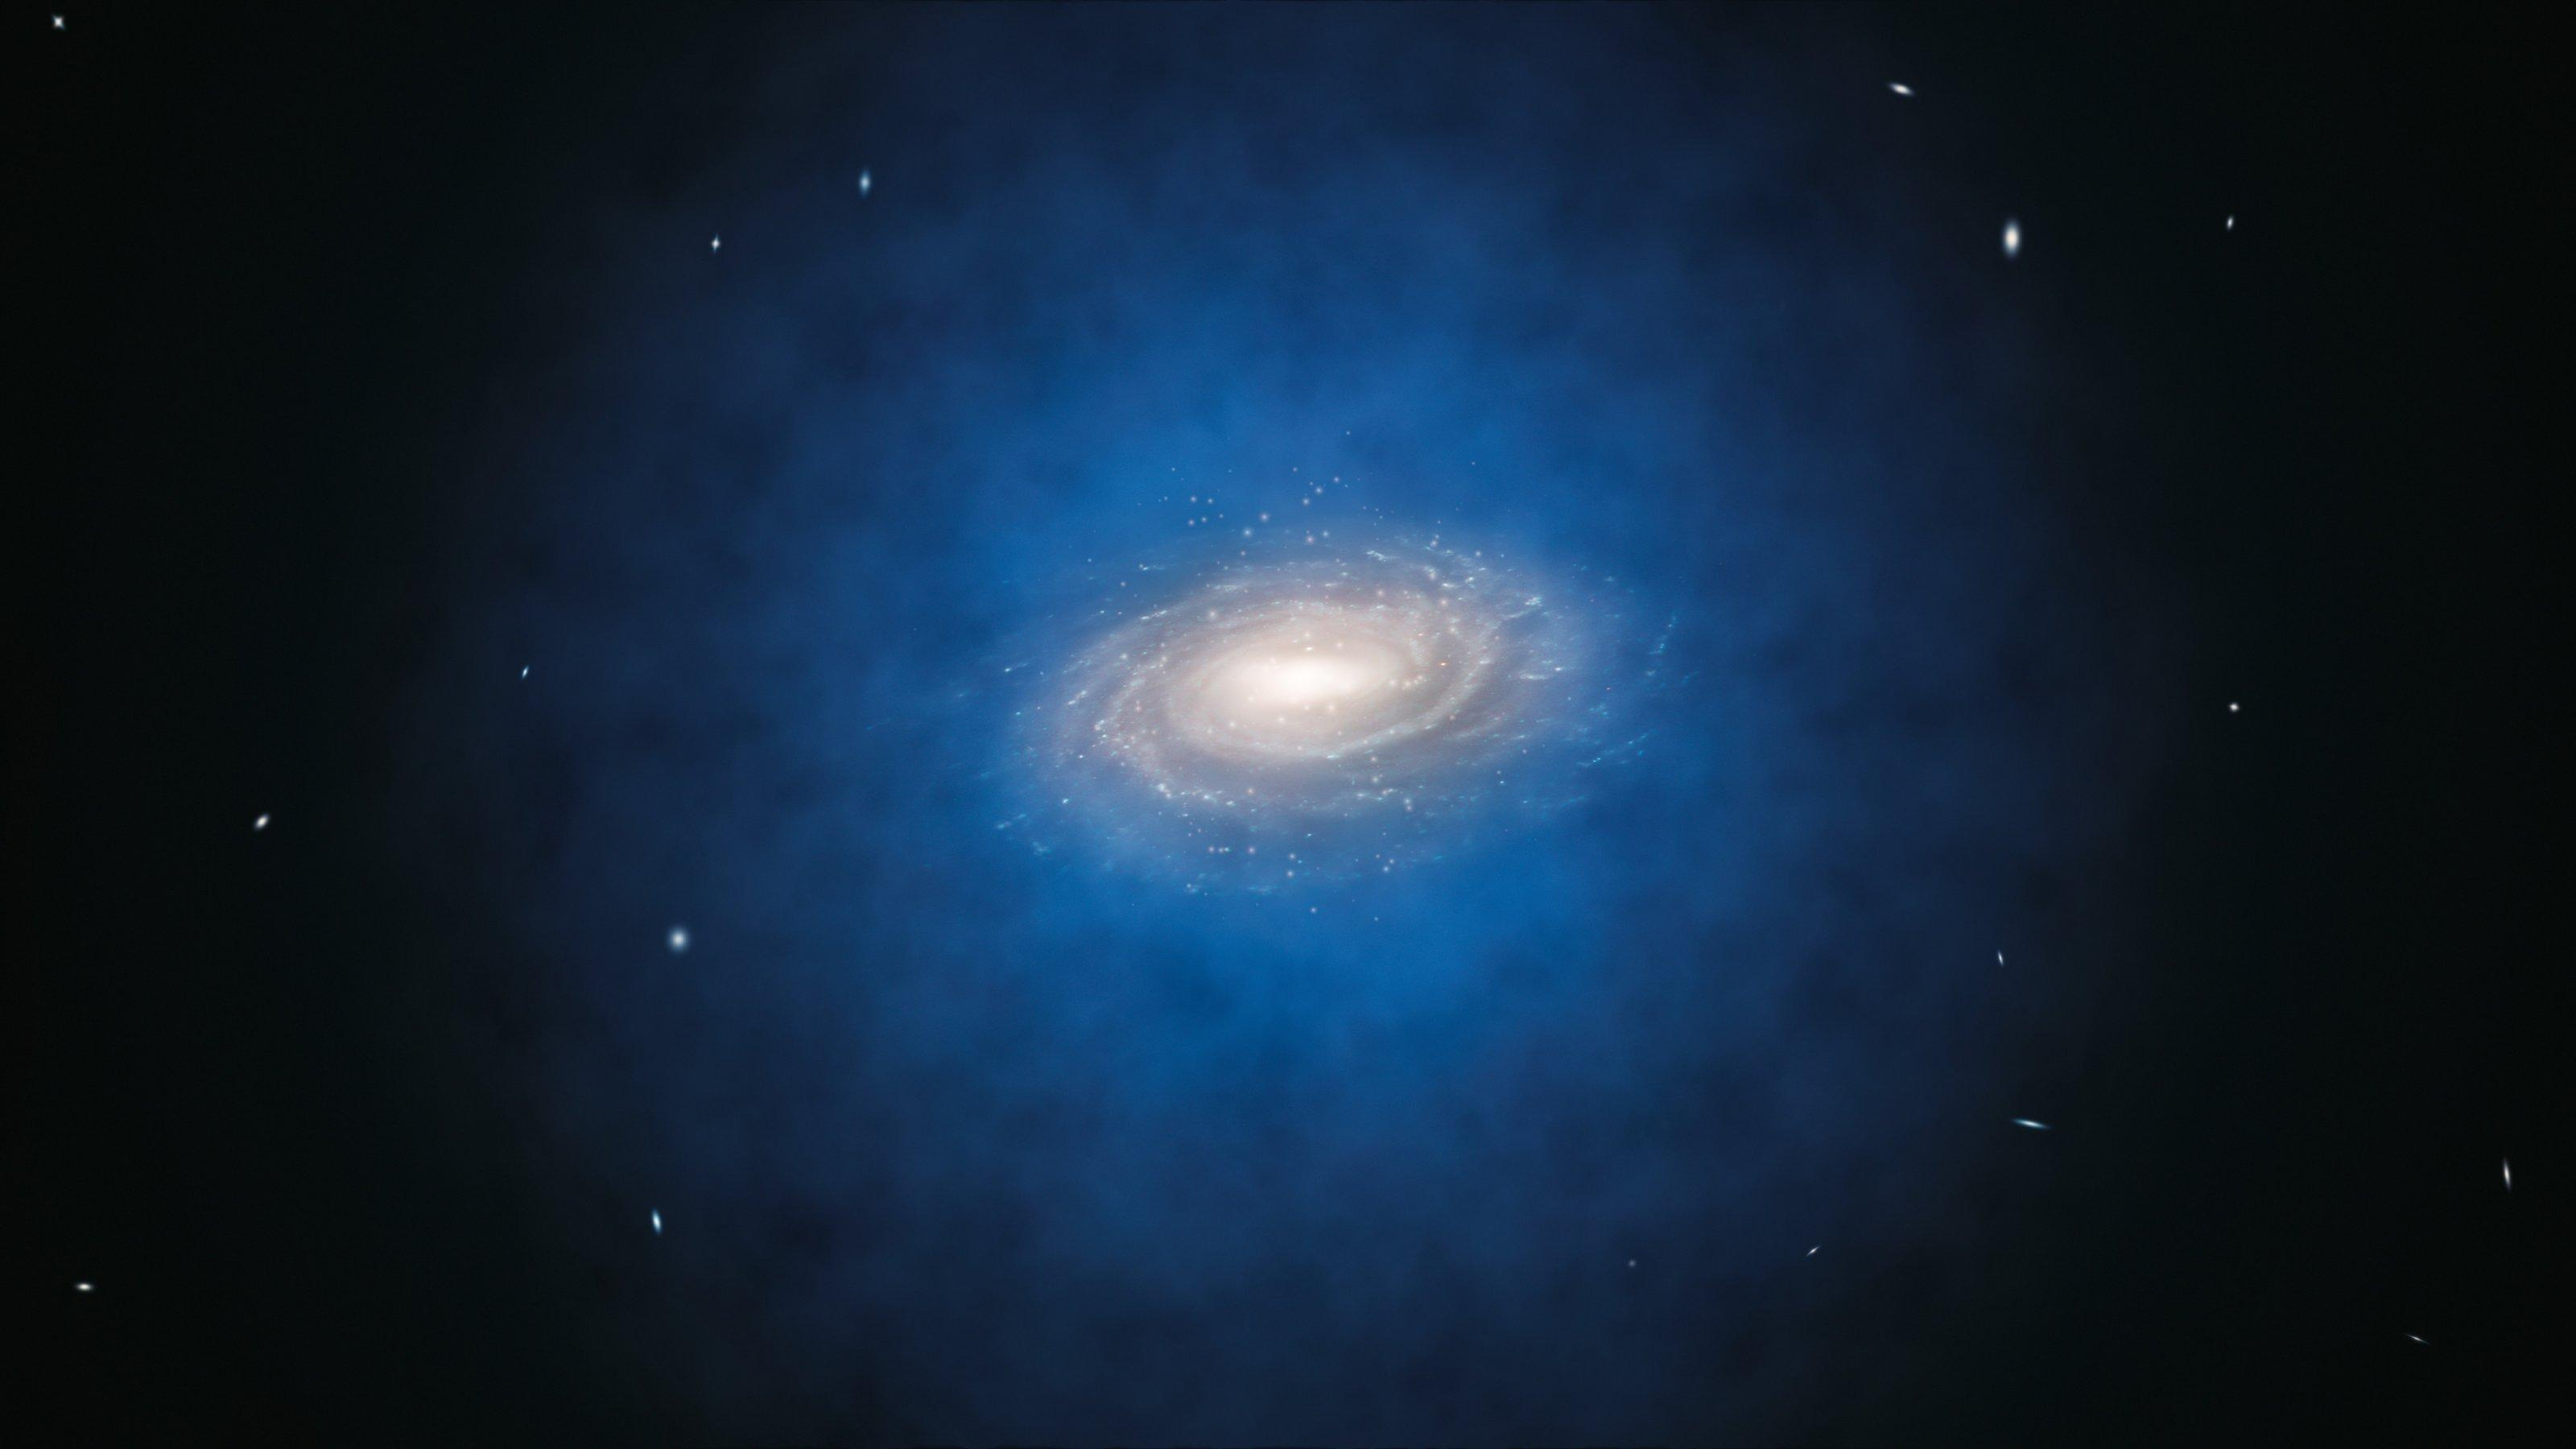
\includegraphics[width=0.6\textwidth]{figures/dark_matter_halo.jpg}
	\caption[Abbildung 3: Dunkle Materie Halo der Milchstrasse]{Veranschaulichung des Dunklen-Materie-Halos der Milchstrasse \cite{Bührke2022}}
	\label{fig Dunkle Materie Halo}
\end{figure}

\subsection{Zusammenhang}

Wenn die Masse einer Galaxie allein aufgrund der sichtbaren Materie (Sterne, Gas und Staub) berechnet wird, kann die erwartete Rotationskurve vorhergesagt werden, diese nimmt mit zunehmender Entfernung vom Zentrum ab. 
Wenn Astronom/innen jedoch tatsächlich die Rota-\\tionsgeschwindigkeit von Sternen und Gas in Galaxien messen, stellen sie fest, dass die beobachteten Rotationskurven von den erwarteten Rotationskurven abweichen.
Anstatt abzunehmen, zeigen die beobachteten Rotationskurven, dass die Rotationsgeschwindigkeit konstant bleibt oder sogar mit zunehmender Entfernung vom Zentrum ansteigt. Die Abweichung zwischen den erwarteten und beobachteten Rotationskurven von Galaxien kann durch die Existenz von Dunkler Materie erklärt werden. 
Die Dunkle Materie erhöht die Massendichte in den äusseren Bereichen von Galaxien und trägt dazu bei, dass die Rotationsgeschwindigkeiten in diesen Bereichen konstant bleiben oder sogar ansteigen.


